%%%%%%%%%%%%%%%%%%%%%%%%%%%%%%%%%%%%%%%%%
% Modified from https://github.com/magicwenli/latex-template-mwhw
%%%%%%%%%%%%%%%%%%%%%%%%%%%%%%%%%%%%%%%%%

\documentclass[12pt,cn]{homework}

% Norm enhanced. Use \norm{}
\newcommand{\norm}[1]{\left\lVert#1\right\rVert}

\usepackage{newtxtext}  % for text fonts
%\setmainfont{Times New Roman}

\usepackage{fontspec}  % for Consolas and Courier New
\lstset{basicstyle=\footnotesize\fontspec{Consolas}}   %Consolas Courier New

%------------------------------------------------------------
%	ASSIGNMENT INFORMATION
%------------------------------------------------------------


%\title{Homework \#1} % Assignment title
\title{Homework}

\author{学生名字} % Student name

%\date{\today} % Due date
\date{2021年X月X日}

\institute{上海师范大学数理学院} % Institute or school name

%\class{微分方程数值 解} % Uncomment for Course or class name

%\professor{教授名字} % Uncomment for Professor or teacher in charge of the assignment

\IDnumber{123002584} % Uncomment for ID in charge of the assignment

\Major{计算数学} % Uncomment for classID in charge of the assignment

\graphicspath{{figures/}}
%------------------------------------------------------------

\begin{document}

\maketitle % Output the assignment title, created automatically using the information in the custom commands above

%------------------------------------------------------------
%	ASSIGNMENT CONTENT
%------------------------------------------------------------

%\section*{问题}


\begin{problem}
证明:范数$\norm{\cdot}$的对偶范数满足范数的定义
	\begin{equation*}
	    \norm{z}_*=\sup\{z^Tx:\ \norm{x}\leq1\}=\sup\{z^Tx:\ \norm{x}=1\}
	\end{equation*}
\end{problem}
\begin{proof}
\begin{equation*}
        \norm{z}_*=\max_{\norm{x}\leq 1}\sum{z_ix_i}
    \end{equation*}
    \begin{enumerate}
    \item 正定性:
    如果$z=0$,显然$\norm{0}_*=0$.
    \item 非负性:
    如果$z\neq 0$,则$\norm{x}\neq 0$. 由于$x=\frac{z}{\norm{z}}$,有$\norm{z}_*\leq \frac{\norm{z}^2_2}{\norm{z}}>0$.\\
    特别的,如果$\norm{z}_*=0$,则必有$z=0$.
    \item 齐次性:\\
    由范数定义,有:
    \begin{equation*}
        \norm{tz}_*=\max_{\norm{x}\leq 1} | z^Ttx|=\max_{\norm{x}\leq 1}|t||z^Tx |=|t| \max_{\norm{x}\leq 1} | z^Tx |=|t|\norm{z}_*
    \end{equation*}
    \end{enumerate}
\end{proof}


%------------------------------------------------------------

\begin{problem}
	这里是一个问题。
\end{problem}
\begin{solution}
这里是问题的解答。
\end{solution}




%------------------------------------------------------------

\clearpage

%\subsection*{表格}
\noindent\textbf{表格}

\begin{table}[ht!]
\caption{表格名字}
\label{tab:3}
\centering
\begin{tabular}{lllllll}
\toprule
  A & N=3 &N=5 & N=7 & N=9 & N=11 & N=13\\
\midrule
  B & 1.5789 & 1.3478 &1.0645&0.8780 &0.7222 &0.5942   \\
   C &  1.0000 &1.0000 &1.0000 &1.0000 &1.0000 &1.0000  \\
D &7.2632 &14.3913 &21.0323 &27.3171 &30.9630 &34.0870   \\
\bottomrule
\end{tabular}
\end{table}


%\subsection*{图片}
\noindent\textbf{图片}

\begin{figure}[htp!]
\centering
  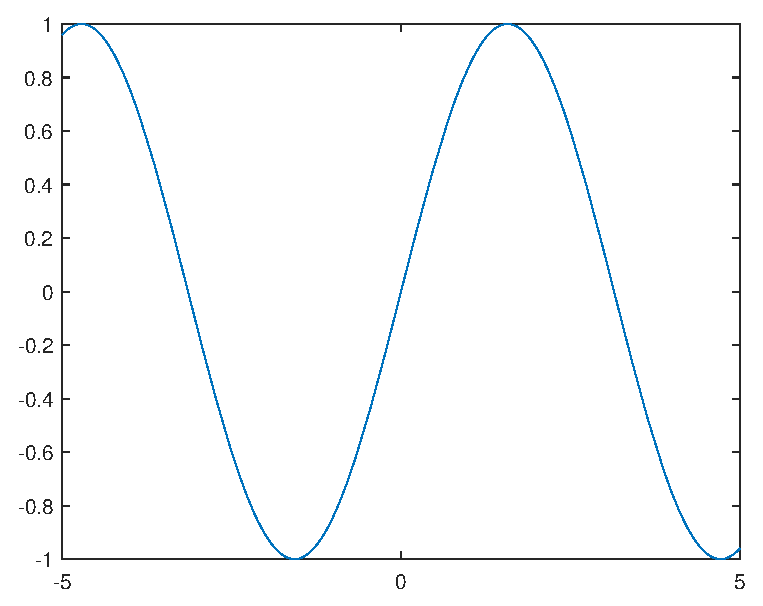
\includegraphics[width=0.6\textwidth]{image1}
   \caption{Euler 方法的误差}
   \label{fig:error1}
\end{figure}


\begin{figure}[!htp]
\begin{minipage}[h]{0.48\linewidth}
\centering
%\captionsetup{width=0.9\linewidth}
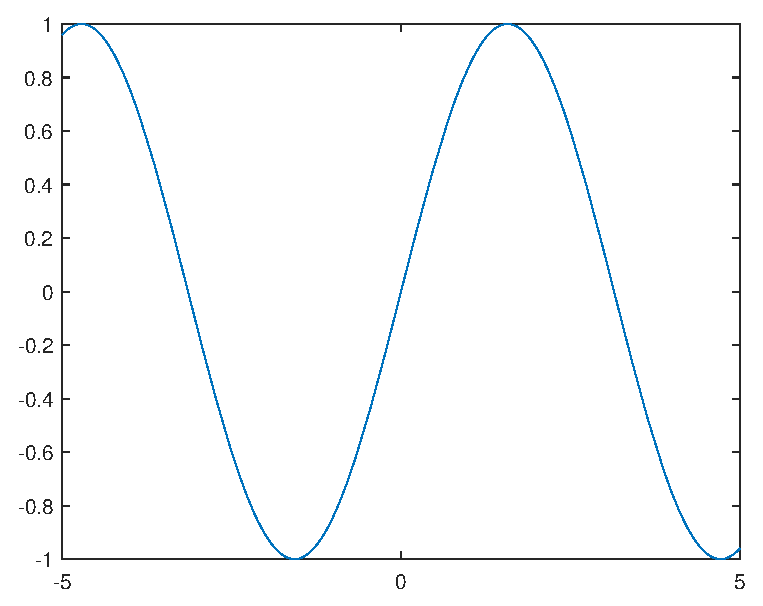
\includegraphics[width=0.9\textwidth]{image1}
\caption{Euler method}
\label{Testfun1}
\end{minipage}
\begin{minipage}[h]{0.48\linewidth}
\centering
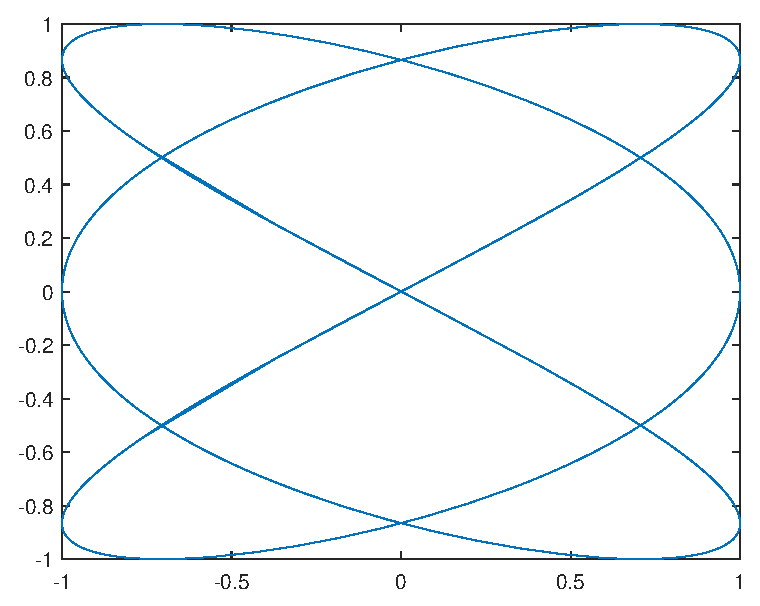
\includegraphics[width=0.9\textwidth]{image2}
\caption{Runge-Kutta method}
\label{Texstfun2}
\end{minipage}
\end{figure}


\clearpage
%\subsection*{MATLAB 代码}
\noindent\textbf{MATLAB 代码}

\begin{lstlisting}[title={Euler method}]
% Euler method for the ODE model
% u'(t)=t^2+t-u, t in [0,1]
% Initial condition: u(0)=0 ;
% Exact solution: u(t)=-exp(-t)+t^2-t+1.
clear all;  clf
h=0.1;
x=0:h:1;                       % function interval
n=length(x)-1;
u(1)=0;                        % initial value
fun=@(t,u) t.^2+t-u;           % RHS
for i=1:n
    u(i+1)=u(i)+h.*fun(x(i),u(i));
end
ue=-exp(-x)+x.^2-x+1;          % exact solution
plot(x,ue,'b-',x,u,'r+','LineWidth',1)
xlabel('x','fontsize', 16), ylabel('y','fontsize',16,'Rotation',0)
set(gca,'fontsize',14)
\end{lstlisting}


\begin{lstlisting}[title={Runge-Kutta method}]
% Runge-Kutta method for the ODE model
% u'=t^2+t-u,  t \in [0,1]
% Initial condition : u(0)=0
% Exact : u(t)=-exp(-t)+t^2-t+1.
clear all;  clf
h=0.1;
x=0:h:1;                     % function interval
n=length(x)-1;
u(1)=0;                      % initial value
fun=@(t,u) t.^2+t-u;         % RHS
for i=1:n
    k1=fun(x(i),u(i));
    k2=fun(x(i)+h./2,u(i)+h.*k1/2);
    k3=fun(x(i)+h./2,u(i)+h.*k2/2);
    k4=fun(x(i)+h,u(i)+h.*k3);
    u(i+1)=u(i)+h.*(k1+2.*k2+2.*k3+k4)./6;
end
ue=-exp(-x)+x.^2-x+1;        % exact solution
plot(x,ue,'b-',x,u,'r+','LineWidth',1)
xlabel('x','fontsize', 16), ylabel('y','fontsize',16)
set(gca,'fontsize',14)
\end{lstlisting}


\end{document}


